\documentclass[
  shownotes,
  xcolor={svgnames},
  hyperref={colorlinks,citecolor=DarkBlue,linkcolor=DarkRed,urlcolor=DarkBlue}
  , aspectratio=169]{beamer}
\usepackage{animate}
\usepackage{amsmath}
\usepackage{amsfonts}
\usepackage{amssymb}
\usepackage{pifont}
\usepackage{mathpazo}
%\usepackage{xcolor}
\usepackage{multimedia}
\usepackage{fancybox}
\usepackage[para]{threeparttable}
\usepackage{multirow}
\setcounter{MaxMatrixCols}{30}
\usepackage{subcaption}
\usepackage{graphicx}
\usepackage{lscape}
\usepackage[compatibility=false,font=small]{caption}
\usepackage{booktabs}
\usepackage{ragged2e}
\usepackage{chronosys}
\usepackage{appendixnumberbeamer}
\usepackage{animate}
\setbeamertemplate{caption}[numbered]
\usepackage{color}
%\usepackage{times}
\usepackage{tikz}
\usepackage{comment} %to comment
%% BibTeX settings
\usepackage{natbib}
\bibliographystyle{apalike}
\bibpunct{(}{)}{,}{a}{,}{,}
\setbeamertemplate{bibliography item}{[\theenumiv]}

% Defines columns for bespoke tables
\usepackage{array}
\newcolumntype{L}[1]{>{\raggedright\let\newline\\\arraybackslash\hspace{0pt}}m{#1}}
\newcolumntype{C}[1]{>{\centering\let\newline\\\arraybackslash\hspace{0pt}}m{#1}}
\newcolumntype{R}[1]{>{\raggedleft\let\newline\\\arraybackslash\hspace{0pt}}m{#1}}


\usepackage{xfrac}


\usepackage{multicol}
\setlength{\columnsep}{0.5cm}

% Theme and colors
\usetheme{Boadilla}

% I use steel blue and a custom color palette. This defines it.
\definecolor{andesred}{HTML}{af2433}

% Other options
\providecommand{\U}[1]{\protect\rule{.1in}{.1in}}
\usefonttheme{serif}
\setbeamertemplate{itemize items}[default]
\setbeamertemplate{enumerate items}[square]
\setbeamertemplate{section in toc}[circle]

\makeatletter

\definecolor{mybackground}{HTML}{82CAFA}
\definecolor{myforeground}{HTML}{0000A0}

\setbeamercolor{normal text}{fg=black,bg=white}
\setbeamercolor{alerted text}{fg=red}
\setbeamercolor{example text}{fg=black}

\setbeamercolor{background canvas}{fg=myforeground, bg=white}
\setbeamercolor{background}{fg=myforeground, bg=mybackground}

\setbeamercolor{palette primary}{fg=black, bg=gray!30!white}
\setbeamercolor{palette secondary}{fg=black, bg=gray!20!white}
\setbeamercolor{palette tertiary}{fg=white, bg=andesred}

\setbeamercolor{frametitle}{fg=andesred}
\setbeamercolor{title}{fg=andesred}
\setbeamercolor{block title}{fg=andesred}
\setbeamercolor{itemize item}{fg=andesred}
\setbeamercolor{itemize subitem}{fg=andesred}
\setbeamercolor{itemize subsubitem}{fg=andesred}
\setbeamercolor{enumerate item}{fg=andesred}
\setbeamercolor{item projected}{bg=gray!30!white,fg=andesred}
\setbeamercolor{enumerate subitem}{fg=andesred}
\setbeamercolor{section number projected}{bg=gray!30!white,fg=andesred}
\setbeamercolor{section in toc}{fg=andesred}
\setbeamercolor{caption name}{fg=andesred}
\setbeamercolor{button}{bg=gray!30!white,fg=andesred}


\usepackage{fancyvrb}
\newcommand{\VerbBar}{|}
\newcommand{\VERB}{\Verb[commandchars=\\\{\}]}
\DefineVerbatimEnvironment{Highlighting}{Verbatim}{commandchars=\\\{\}}
% Add ',fontsize=\small' for more characters per line
\usepackage{framed}
\definecolor{shadecolor}{RGB}{248,248,248}
\newenvironment{Shaded}{\begin{snugshade}}{\end{snugshade}}
\newcommand{\AlertTok}[1]{\textcolor[rgb]{0.94,0.16,0.16}{#1}}
\newcommand{\AnnotationTok}[1]{\textcolor[rgb]{0.56,0.35,0.01}{\textbf{\textit{#1}}}}
\newcommand{\AttributeTok}[1]{\textcolor[rgb]{0.77,0.63,0.00}{#1}}
\newcommand{\BaseNTok}[1]{\textcolor[rgb]{0.00,0.00,0.81}{#1}}
\newcommand{\BuiltInTok}[1]{#1}
\newcommand{\CharTok}[1]{\textcolor[rgb]{0.31,0.60,0.02}{#1}}
\newcommand{\CommentTok}[1]{\textcolor[rgb]{0.56,0.35,0.01}{\textit{#1}}}
\newcommand{\CommentVarTok}[1]{\textcolor[rgb]{0.56,0.35,0.01}{\textbf{\textit{#1}}}}
\newcommand{\ConstantTok}[1]{\textcolor[rgb]{0.00,0.00,0.00}{#1}}
\newcommand{\ControlFlowTok}[1]{\textcolor[rgb]{0.13,0.29,0.53}{\textbf{#1}}}
\newcommand{\DataTypeTok}[1]{\textcolor[rgb]{0.13,0.29,0.53}{#1}}
\newcommand{\DecValTok}[1]{\textcolor[rgb]{0.00,0.00,0.81}{#1}}
\newcommand{\DocumentationTok}[1]{\textcolor[rgb]{0.56,0.35,0.01}{\textbf{\textit{#1}}}}
\newcommand{\ErrorTok}[1]{\textcolor[rgb]{0.64,0.00,0.00}{\textbf{#1}}}
\newcommand{\ExtensionTok}[1]{#1}
\newcommand{\FloatTok}[1]{\textcolor[rgb]{0.00,0.00,0.81}{#1}}
\newcommand{\FunctionTok}[1]{\textcolor[rgb]{0.00,0.00,0.00}{#1}}
\newcommand{\ImportTok}[1]{#1}
\newcommand{\InformationTok}[1]{\textcolor[rgb]{0.56,0.35,0.01}{\textbf{\textit{#1}}}}
\newcommand{\KeywordTok}[1]{\textcolor[rgb]{0.13,0.29,0.53}{\textbf{#1}}}
\newcommand{\NormalTok}[1]{#1}
\newcommand{\OperatorTok}[1]{\textcolor[rgb]{0.81,0.36,0.00}{\textbf{#1}}}
\newcommand{\OtherTok}[1]{\textcolor[rgb]{0.56,0.35,0.01}{#1}}
\newcommand{\PreprocessorTok}[1]{\textcolor[rgb]{0.56,0.35,0.01}{\textit{#1}}}
\newcommand{\RegionMarkerTok}[1]{#1}
\newcommand{\SpecialCharTok}[1]{\textcolor[rgb]{0.00,0.00,0.00}{#1}}
\newcommand{\SpecialStringTok}[1]{\textcolor[rgb]{0.31,0.60,0.02}{#1}}
\newcommand{\StringTok}[1]{\textcolor[rgb]{0.31,0.60,0.02}{#1}}
\newcommand{\VariableTok}[1]{\textcolor[rgb]{0.00,0.00,0.00}{#1}}
\newcommand{\VerbatimStringTok}[1]{\textcolor[rgb]{0.31,0.60,0.02}{#1}}
\newcommand{\WarningTok}[1]{\textcolor[rgb]{0.56,0.35,0.01}{\textbf{\textit{#1}}}}
\usepackage{graphicx}
\makeatletter


% colors
\definecolor{airforceblue}{rgb}{0.36, 0.54, 0.66}
\newcommand{\theme}{\color{andesred}}
\newcommand{\bk}{\color{black}}
\newcommand{\rd}{\color{red}}
\newcommand{\fg}{\color{ForestGreen}}
\newcommand{\bl}{\color{blue}}
\newcommand{\gr}{\color{black!60}}
\newcommand{\sg}{\color{DarkSlateGray}}
\newcommand{\br}{\color{SaddleBrown}}
\newcommand{\nv}{\color{Navy}}


% common math markups
\newcommand{\bs}[1]{\boldsymbol{#1}}
\newcommand{\mc}[1]{\mathcal{#1}}
\newcommand{\mr}[1]{\mathrm{#1}}
\newcommand{\bm}[1]{\mathbf{#1}}
\newcommand{\ds}[1]{\mathds{#1}}
\newcommand{\indep}{\perp\!\!\!\perp}

% shorthand
\newcommand{\sk}{\vspace{.5cm}}
\newcommand{\R}[1]{{\tt \nv #1}}
\newcommand{\til}{{\footnotesize$\bs{\stackrel{\sim}{}}$}}
\DeclareSymbolFont{extraup}{U}{zavm}{m}{n}
\DeclareMathSymbol{\vardiamond}{\mathalpha}{extraup}{87}


\usepackage{tikz}
% Tikz settings optimized for causal graphs.
\usetikzlibrary{shapes,decorations,arrows,calc,arrows.meta,fit,positioning}
\tikzset{
    -Latex,auto,node distance =1 cm and 1 cm,semithick,
    state/.style ={ellipse, draw, minimum width = 0.7 cm},
    point/.style = {circle, draw, inner sep=0.04cm,fill,node contents={}},
    bidirected/.style={Latex-Latex,dashed},
    el/.style = {inner sep=2pt, align=left, sloped}
}


\makeatother






%%%%%%%%%%%%%%% BEGINS DOCUMENT %%%%%%%%%%%%%%%%%%

\begin{document}
 
\title[Lecture 26]{Lecture 26:  XGBoost \& Text as Data}
\subtitle{Big Data and Machine Learning for Applied Economics \\ Econ 4676}
\date{\today}

\author[Sarmiento-Barbieri]{Ignacio Sarmiento-Barbieri}
\institute[Uniandes]{Universidad de los Andes}


\begin{frame}[noframenumbering]
\maketitle
\end{frame}

%%%%%%%%%%%%%%%%%%%%%%%%%%%%%%%%%%%




%----------------------------------------------------------------------% 

\begin{frame}
\frametitle{Agenda}

\tableofcontents

\end{frame}
%----------------------------------------------------------------------%
\section{Recap: XGBoost}
%----------------------------------------------------------------------%
\begin{frame}[fragile]
\frametitle{XGBoost: Recap}

\begin{itemize}

\item Why talk about XGBoost?
\begin{itemize}


 \item Among the 29 challenge winning solutions published in Kaggle's blog during 2015, 17 solutions used XGBoost.  
 \medskip
 \item Among these solutions,  eight  solely  used  XGBoost  to  train  the  model, while most others combined XGBoost with neural nets in ensembles. (The second most popular method, deep  neural  nets,  was  used  in  11  solutions) 
 \medskip
 \item   The  success of the system was also witnessed in 2015 Data Mining and Knowledge Discovery competition organized by ACM (KDD Cup) , where XGBoost  was  used  by  every  winning  team  in  the  top-10. 
 \medskip
 \item Historically, XGBoost has performed quite well for structured, tabular data. But, if you are dealing with non-structured data such as images, neural networks are usually a better option (more on this later)
\end{itemize}
 \end{itemize}
\end{frame}


%----------------------------------------------------------------------%
\begin{frame}[fragile]
\frametitle{Boosting Trees}


\begin{itemize}
\item Learning tree structure is much harder than traditional optimization problem where you can simply take the gradient. 
\item It is intractable to learn all the trees at once. 
\item Instead, we use an additive strategy: fix what we have learned, and add one new tree at a time. We write the prediction value at step m as $\hat{y}_i^{m}$. 
\item Then we have
\begin{align}
\hat{y}_i^{0} &=0 \\ \nonumber
\hat{y}_i^{1} &= \hat{y}_i^{0} + f_1(x_i) \\ \nonumber
\hat{y}_i^{2} &= \hat{y}_i^{1} + f_2(x_i) \\ \nonumber
\dots \\ \nonumber
\hat{y}_i^{M} &= \sum_{m=1}^M f_m(x_i) = \hat{y}_i^{m-1} + f_m(x_i) \\ \nonumber
\end{align}
\end{itemize}


 \end{frame}
%----------------------------------------------------------------------%
\begin{frame}[fragile]
\frametitle{XGBoost is a Boosting Tree }

\begin{itemize}


\item Which tree do we want at each step? 
\item Add the one that optimizes our objective.

\begin{align}
\mathcal{L} &= \sum_{i=1}^N L(y_i,\hat{y}_i) + \sum_{k=1}^m \Omega(f_k)
\end{align}

\item  $L(.)$ is a differentiable convex loss function that measures the difference between the prediction $\hat{y}_i$ and the target $y_i$. 
\item  The second term $\Omega(f)$ penalizes the complexity of the model, where


\begin{align}
\Omega(f)=\gamma T + \frac{1}{2}\lambda ||\omega||_2
\end{align}


\end{itemize}
 \end{frame}
%----------------------------------------------------------------------%
\begin{frame}[fragile]
\frametitle{XGBoost is a Boosting Tree }

\begin{itemize}
\item The fuction above cannot be optimized using traditional optimization methods
\item Let $\mathcal{L}^m$ be the loss at step $m$, then $\hat{y}_i^m$ is the prediction of row $i$ at the $m$ iteration
\item We need to add $f_m$ to minimize the following objective
  \begin{align}
\mathcal{L}^m=\sum_{i=1}^N (y_i-\hat{y}_i^{m-1} + f_m(x_i))^2  +  \Omega(f_t)
\end{align}

\item  So in the general case, we take a second order  Taylor expansion of the loss function:

\begin{align}
\mathcal{L}^m &= \sum_{i=1}^N \left[ L(y_i,\hat{y}_i^{(m-1)}) + r_{im} f_m(x_i) + \frac{1}{2}h_i f^2_m(x_i) \right] +  \Omega(f_t)
\end{align}

where  $r_{im} = \frac{\partial L(y_i,\hat{y}_i^{(m-1)})}{\partial f^{(m-1)}(\mathbf{x}_i)}$ and $h_{im} = \frac{\partial^2 L(y_i,\hat{y}_i^{(m-1)})}{\partial (f^{(m-1)}(\mathbf{x}_i))^2}$
  \end{itemize}
 \end{frame}
%----------------------------------------------------------------------%
\begin{frame}[fragile]
\frametitle{XGBoost is a Boosting Tree }

\begin{itemize}


\item After we remove all the constants, the specific objective at step m becomes


\begin{align}
\mathcal{L}^m &= \sum_{i=1}^N \left[ r_{im} f_m(x_i) + \frac{1}{2}h_i f^2_m(x_i) \right] +  \Omega(f_t)
\end{align}

\item This becomes our optimization goal for the new tree. One important advantage of this definition is that the value of the objective function only depends on $r_{im}$ and $h_{im}$ 


\end{itemize}



 \end{frame}

%----------------------------------------------------------------------%
\begin{frame}[fragile]
\frametitle{XGBoost Model Complexity}

\begin{itemize}
\item Let's talk about the  regularization term 
\item We need to define the complexity of the tree $\Omega(f)$.
\item But us first refine the definition of the tree $f(x)$ as

 
\begin{align}
f_t(x) = w_{q(x)}, w \in R^T, q:R^d\rightarrow \{1,2,\cdots,T\} .
\end{align}


\item Here $w$ is the vector of predictions on leaves, $q$ is a function assigning each data point to the corresponding leaf, and $T$ is the number of leaves. 


\item In XGBoost, they define the complexity as
\begin{align}
\Omega(f) = \gamma T + \frac{1}{2}\lambda \sum_{j=1}^T w_j^2
\end{align}


\end{itemize}
 \end{frame}

%----------------------------------------------------------------------%
\begin{frame}[fragile]
\frametitle{XGBoost Model Complexity}

\begin{itemize}
\item With the aboe notation we can re writ the objective funtion as 


\begin{align}
\mathcal{L}^{(t)} &\approx \sum_{i=1}^n [g_i w_{q(x_i)} + \frac{1}{2} h_i w_{q(x_i)}^2] + \gamma T + \frac{1}{2}\lambda \sum_{j=1}^T w_j^2\\
&= \sum^T_{j=1} [(\sum_{i\in I_j} g_i) w_j + \frac{1}{2} (\sum_{i\in I_j} h_i + \lambda) w_j^2 ] + \gamma T\
\end{align}

\item where $I_j={i|q(x_i)=j}$ set of indicators that assign to the $j-th$ leaf.
\item Note the following in the second line, we changed the index of the summation because all the data points on the smae leaf get the same score.
\item Defining $G_j = \sum_{i\in I_j} g_i$ and $H_j = \sum_{i\in I_j} h_i$

\begin{align}
\mathcal{L}^{(t)} = \sum^T_{j=1} [G_jw_j + \frac{1}{2} (H_j+\lambda) w_j^2] +\gamma T
\end{align}

\end{itemize}

\end{frame}

%----------------------------------------------------------------------%
\begin{frame}[fragile]
\frametitle{XGBoost Model Complexity}

\begin{itemize}
\item In the above equation, $w_j$ are independent with respect to each other, 
\item the form $G_jw_j+\frac{1}{2}(H_j+\lambda)w_j^2$  is quadratic 
\item then the best $w_j$ for a given structure tree structure $q(x)$ get is:


\begin{align}
w_j^\ast &= -\frac{G_j}{H_j+\lambda}\\
\end{align}


\item and the best objective reduction we can get

\begin{align}
\mathcal{L}^\ast &= -\frac{1}{2} \sum_{j=1}^T \frac{G_j^2}{H_j+\lambda} + \gamma T
\end{align}

\end{itemize}



 

\end{frame}
%----------------------------------------------------------------------%
\begin{frame}[fragile]
\frametitle{XGBoost Model Complexity: Example}
  \begin{figure}[H] \centering
            \captionsetup{justification=centering}
              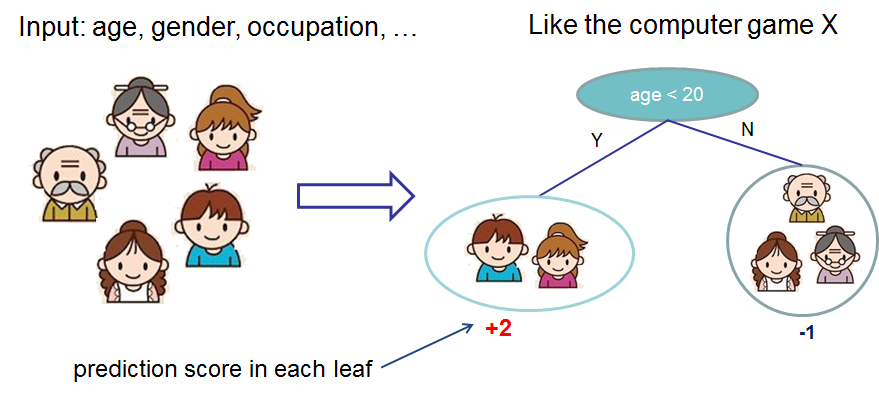
\includegraphics[scale=0.6]{figures/cart}
              \\
              \tiny
              \url{source: https://xgboost.readthedocs.io/en/latest/tutorials/model.html}
 \end{figure}

\end{frame}
%----------------------------------------------------------------------%
\begin{frame}[fragile]
\frametitle{XGBoost Model Complexity: Example}
  \begin{figure}[H] \centering
            \captionsetup{justification=centering}
              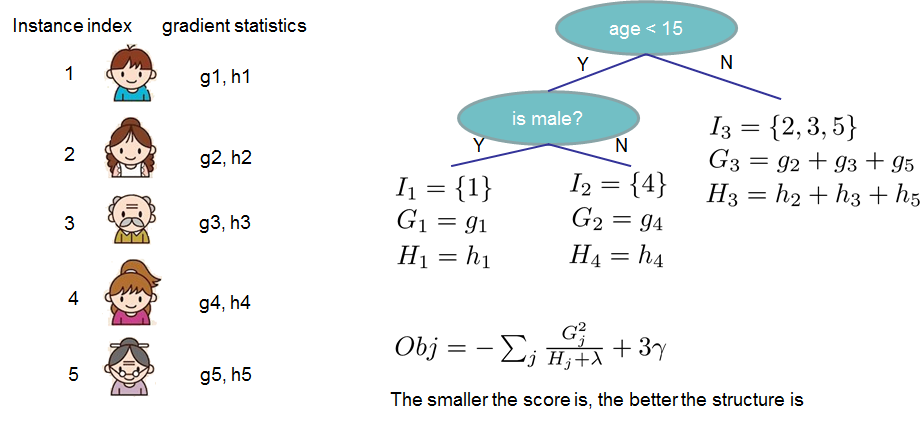
\includegraphics[scale=0.6]{figures/struct_score}
              \\
              \tiny
              \url{source: https://xgboost.readthedocs.io/en/latest/tutorials/model.html}
 \end{figure}

 \end{frame}
%----------------------------------------------------------------------%
\begin{frame}[fragile]
\frametitle{Learn the tree structure}



Now that we have a way to measure how good a tree is, ideally we would enumerate all possible trees and pick the best one. In practice this is intractable, so we will try to optimize one level of the tree at a time. Specifically we try to split a leaf into two leaves, and the score it gains is

\begin{align}
Gain = \frac{1}{2} \left[\frac{G_L^2}{H_L+\lambda}+\frac{G_R^2}{H_R+\lambda}-\frac{(G_L+G_R)^2}{H_L+H_R+\lambda}\right] - \gamma
\end{align}

 \end{frame}
%----------------------------------------------------------------------%
\begin{frame}[fragile]
\frametitle{Learn the tree structure}

\begin{itemize}
  \item This formula can be decomposed as 
\begin{enumerate}
\item  the score on the new left leaf 
\item the score on the new right leaf 
\item The score on the original leaf 
\item  regularization on the additional leaf. 
\end{enumerate}
\item We can see an important fact here: if the gain is smaller than $\gamma$ , we would do better not to add that branch. This is exactly the pruning techniques in tree based models

\item For real valued data, we usually want to search for an optimal split. To efficiently do so, we place all the instances in sorted order

\item A left to right scan is sufficient to calculate the structure score of all possible split solutions, and we can find the best split efficiently
\end{itemize}

\end{frame}
%----------------------------------------------------------------------%
\begin{frame}[fragile]
\frametitle{Learn the tree structure}

  \begin{figure}[H] \centering
            \captionsetup{justification=centering}
              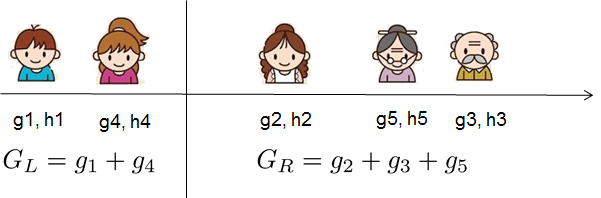
\includegraphics[scale=0.6]{figures/tree_structure}
              \\
              \tiny
              \url{source: https://xgboost.readthedocs.io/en/latest/tutorials/model.html}
 \end{figure}
 
\end{frame}


%----------------------------------------------------------------------%
\subsection{XGBoost: Demo}
%----------------------------------------------------------------------%
\begin{frame}[fragile]
\frametitle{XGBoost: Demo}



\begin{Shaded}
\begin{Highlighting}[]
\CommentTok{\#Load the required packages}
\KeywordTok{library}\NormalTok{(}\StringTok{"McSpatial"}\NormalTok{) }\CommentTok{\#loads the package}
\KeywordTok{library}\NormalTok{(}\StringTok{"dplyr"}\NormalTok{) }\CommentTok{\#for data wrangling}
\KeywordTok{library}\NormalTok{(}\StringTok{"caret"}\NormalTok{)}

\KeywordTok{data}\NormalTok{(matchdata) }\CommentTok{\#loads the data set}
\KeywordTok{set.seed}\NormalTok{(}\DecValTok{123}\NormalTok{) }\CommentTok{\#set the seed for replication purposes}
\end{Highlighting}
\end{Shaded}

\begin{Shaded}
\begin{Highlighting}[]
\CommentTok{\#linear regression}
\NormalTok{model\_lm\textless{}{-}}\KeywordTok{train}\NormalTok{(lnprice}\OperatorTok{\textasciitilde{}}\NormalTok{.}\OperatorTok{+}\NormalTok{.}\OperatorTok{:}\NormalTok{latitude}\OperatorTok{+}\NormalTok{.}\OperatorTok{:}\NormalTok{longitude}\OperatorTok{+}\NormalTok{.}\OperatorTok{:}\NormalTok{latitude}\OperatorTok{:}\NormalTok{longitude,  }
                     \DataTypeTok{data =}\NormalTok{ matchdata,}
                     \DataTypeTok{trControl =} \KeywordTok{trainControl}\NormalTok{(}\DataTypeTok{method =} \StringTok{"cv"}\NormalTok{, }\DataTypeTok{number =} \DecValTok{5}\NormalTok{), }
                     \DataTypeTok{method =} \StringTok{"lm"}\NormalTok{)    }
\end{Highlighting}
\end{Shaded}

\end{frame}
%----------------------------------------------------------------------%
\begin{frame}[fragile]
\frametitle{XGBoost: Demo}


\begin{Shaded}
\begin{Highlighting}[]
\NormalTok{model\_lm}
\end{Highlighting}
\end{Shaded}

\begin{tiny}
\begin{verbatim}
## Linear Regression 
## 
## 3204 samples
##   17 predictor
## 
## No pre-processing
## Resampling: Cross-Validated (5 fold) 
## Summary of sample sizes: 2562, 2564, 2561, 2564, 2565 
## Resampling results:
## 
##   RMSE       Rsquared   MAE      
##   0.2058519  0.8472526  0.1442374
## 
## Tuning parameter 'intercept' was held constant at a value of TRUE
\end{verbatim}
\end{tiny}
\end{frame}
%----------------------------------------------------------------------%
\begin{frame}[fragile]
\frametitle{XGBoost: Demo}
\begin{itemize}
\item From \texttt{Caret's} manual

\item eXtreme Gradient Boosting
\medskip
\begin{itemize}
\item method = `xgbTree'
\medskip
\item Type: Regression, Classification
\medskip
\item Tuning parameters:

  
  \begin{verbatim}
  nrounds (# Boosting Iterations)
  max_depth (Max Tree Depth)
  eta (Shrinkage)
  gamma (Minimum Loss Reduction)
  colsample_bytree (Subsample Ratio of Columns)
  min_child_weight (Minimum Sum of Instance Weight)
  subsample (Subsample Percentage)
  \end{verbatim}



  \item Required packages: xgboost, plyr
  \medskip
  \item A model-specific variable importance metric is available.
\end{itemize}
\end{itemize}

\end{frame}
%----------------------------------------------------------------------%
\begin{frame}[fragile]
\frametitle{XGBoost: Demo}

\begin{scriptsize}
\begin{Shaded}
\begin{Highlighting}[]

\NormalTok{tune\_grid \textless{}{-}}\StringTok{ }\KeywordTok{expand.grid}\NormalTok{(}
  \DataTypeTok{nrounds =} \KeywordTok{seq}\NormalTok{(}\DataTypeTok{from =} \DecValTok{200}\NormalTok{, }\DataTypeTok{to =} \DecValTok{1000}\NormalTok{, }\DataTypeTok{by =} \DecValTok{50}\NormalTok{),}
  \DataTypeTok{eta =} \KeywordTok{c}\NormalTok{(}\FloatTok{0.025}\NormalTok{, }\FloatTok{0.05}\NormalTok{, }\FloatTok{0.1}\NormalTok{, }\FloatTok{0.3}\NormalTok{),}
  \DataTypeTok{max\_depth =} \KeywordTok{c}\NormalTok{(}\DecValTok{2}\NormalTok{, }\DecValTok{3}\NormalTok{, }\DecValTok{4}\NormalTok{, }\DecValTok{5}\NormalTok{, }\DecValTok{6}\NormalTok{),}
  \DataTypeTok{gamma =} \DecValTok{0}\NormalTok{,}
  \DataTypeTok{colsample\_bytree =} \DecValTok{1}\NormalTok{,}
  \DataTypeTok{min\_child\_weight =} \DecValTok{1}\NormalTok{,}
  \DataTypeTok{subsample =} \DecValTok{1}
\NormalTok{)}

\NormalTok{tune\_control \textless{}{-}}\StringTok{ }\NormalTok{caret}\OperatorTok{::}\KeywordTok{trainControl}\NormalTok{(}
  \DataTypeTok{method =} \StringTok{"cv"}\NormalTok{, }\CommentTok{\# cross{-}validation}
  \DataTypeTok{number =} \DecValTok{3}\NormalTok{, }\CommentTok{\# with n folds }
  \CommentTok{\#index = createFolds(tr\_treated$Id\_clean), \# fix the folds}
  \DataTypeTok{verboseIter =} \OtherTok{FALSE}\NormalTok{, }\CommentTok{\# no training log}
  \DataTypeTok{allowParallel =} \OtherTok{TRUE} \CommentTok{\# FALSE for reproducible results }
\NormalTok{)}
\end{Highlighting}
\end{Shaded}

\end{scriptsize}
\end{frame}
%----------------------------------------------------------------------%
\begin{frame}[fragile]
\frametitle{XGBoost: Demo}

\begin{scriptsize}
\begin{Shaded}
\begin{Highlighting}[]
\NormalTok{input\_x \textless{}{-}}\StringTok{ }\KeywordTok{select}\NormalTok{(matchdata, }\OperatorTok{{-}}\NormalTok{lnprice)}
\NormalTok{input\_x}\OperatorTok{$}\NormalTok{year \textless{}{-}}\KeywordTok{as.factor}\NormalTok{(input\_x}\OperatorTok{$}\NormalTok{year)}
\NormalTok{input\_x}\OperatorTok{$}\NormalTok{carea \textless{}{-}}\KeywordTok{as.factor}\NormalTok{(input\_x}\OperatorTok{$}\NormalTok{carea)}
\KeywordTok{require}\NormalTok{(}\StringTok{"Matrix"}\NormalTok{)}
\end{Highlighting}
\end{Shaded}

\begin{Shaded}
\begin{Highlighting}[]
\NormalTok{input\_x\textless{}{-}}\StringTok{ }\KeywordTok{sparse.model.matrix}\NormalTok{(}\OperatorTok{\textasciitilde{}}\NormalTok{.,}\DataTypeTok{data=}\NormalTok{input\_x)}
\NormalTok{input\_y \textless{}{-}}\StringTok{ }\NormalTok{matchdata}\OperatorTok{$}\NormalTok{lnprice}

\NormalTok{model\_xgb \textless{}{-}}\StringTok{ }\NormalTok{caret}\OperatorTok{::}\KeywordTok{train}\NormalTok{(}
  \DataTypeTok{x =}\NormalTok{ input\_x,}
  \DataTypeTok{y =}\NormalTok{ input\_y,}
  \DataTypeTok{trControl =}\NormalTok{ tune\_control,}
  \DataTypeTok{tuneGrid =}\NormalTok{ tune\_grid,}
  \DataTypeTok{method =} \StringTok{"xgbTree"}\NormalTok{,}
  \DataTypeTok{verbose =} \OtherTok{TRUE}
\NormalTok{)}
\end{Highlighting}
\end{Shaded}


\begin{Shaded}
\begin{Highlighting}[]
\NormalTok{model\_xgb}\OperatorTok{$}\NormalTok{bestTune}
\end{Highlighting}
\end{Shaded}

\begin{verbatim}
##    nrounds max_depth  eta gamma colsample_bytree min_child_weight subsample
## 93     550         2 0.05     0                1                1         1
\end{verbatim}
\end{scriptsize}
\end{frame}
%----------------------------------------------------------------------%
\begin{frame}[fragile]
\frametitle{XGBoost: Demo}



  \begin{figure}[H] \centering
            \captionsetup{justification=centering}
              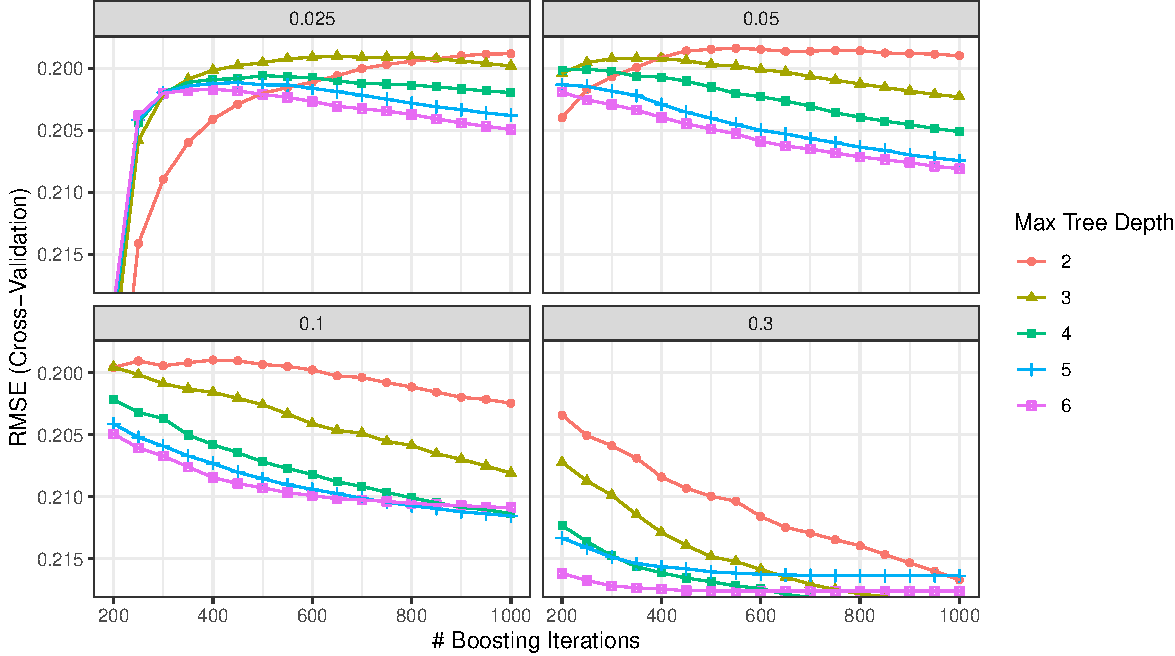
\includegraphics[scale=0.6]{figures/unnamed-chunk-4-1.pdf}
              
 \end{figure}

\end{frame}
%----------------------------------------------------------------------%
\section{Text as Data}
%----------------------------------------------------------------------%
\begin{frame}[fragile]
\frametitle{Text as Data: Motivation}

{\bf We'll start with a story: \theme Slant in Partisan Speech}

  \begin{figure}[H] \centering
            \captionsetup{justification=centering}
              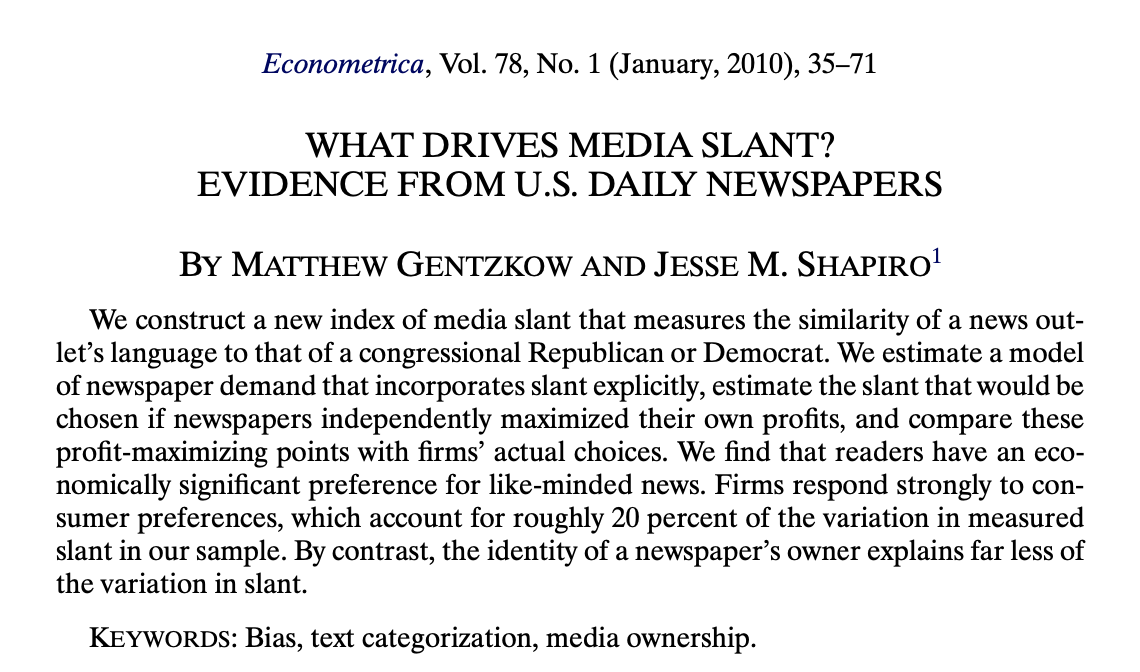
\includegraphics[scale=0.6]{figures/gentzgow_shapiro}
              
 \end{figure}

\end{frame}
%----------------------------------------------------------------------%
\begin{frame}[fragile]
\frametitle{Text as Data: Motivation}
\framesubtitle{Gentzkow and Shapiro: What drives media slant?  Evidence from
U.S. daily newspapers ({\it Econometrica}, 2010)}

\begin{itemize}
\item Build an economic model for newspaper demand that incorporates political partisanship (\rd Republican \bk vs \bl Democrat\bk)


 
\begin{itemize}
\item What would be independent profit-maximizing ``slant''?
\item Compare this to slant estimated from newspaper text.
\end{itemize}
\end{itemize}

\begin{center}
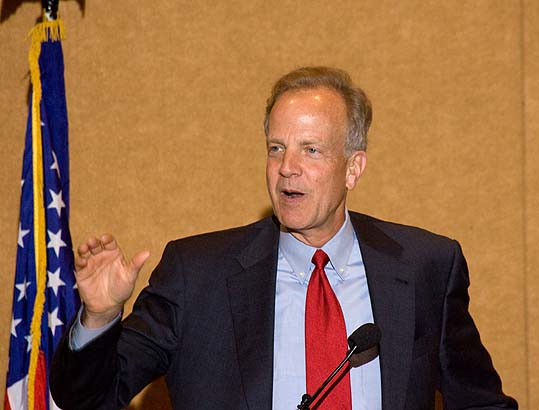
\includegraphics[width=1.7in]{figures/moran}
~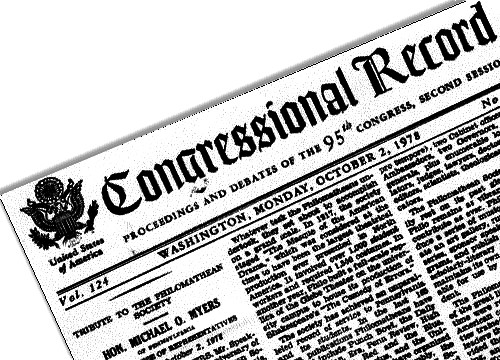
\includegraphics[width=1.75in]{figures/record}
\end{center}


 \end{frame}
%----------------------------------------------------------------------%
\begin{frame}[fragile]
\frametitle{Text as Data: Motivation}

\begin{itemize} 
\item Jerry Moran, R-KS, says ``death tax'' relatively often and his district
(Kansas 1st) voted 73\% for George W. Bush in 2004.
\end{itemize}

\begin{center}
$\bm{X_\text{text}} = f( \text{ideology}) \approx g(Y_{Bush})$

\vskip .25cm
$\bm{\Rightarrow}$ ``death tax'' is republican

\vskip .25cm
$\Rightarrow $ \theme the Wall Street Journal is slanted right.
\end{center}


\end{frame}
%----------------------------------------------------------------------%
\begin{frame}[fragile]
\frametitle{Text as Data: What is slant?}

\begin{itemize}
\item { Text:}  phrase-counts by speaker in 109$^{th}$ US Congress
(05-06)
\medskip
\item  { Sentiment:} two-party constituent vote-share for Bush in 2004.
\medskip

\item  Use covariance between  phrase frequencies ($f_{ij}$) and `Bush' sentiment ($y_i$)  to build an index of partisanship for text. 
\begin{center}\large
$z^{slant}_i= \sum_j \mr{cov}(f_j, y) f_{ij}$
\end{center}
\medskip
 \item For example, if phrase $j$ forms  a high proportion of what you say, and usage of phrase
 \medskip
\item $j$ is correlated with Bush vote-share, then this contributes a positive amount to your slant score.
\medskip
\vskip .2cm
\item  This is a type of {\it marginal regression}.
\end{itemize}
\end{frame}
%----------------------------------------------------------------------%
\begin{frame}[fragile]
\frametitle{Text as Data: Wordle} 


  \begin{figure}[H] \centering
            \captionsetup{justification=centering}
              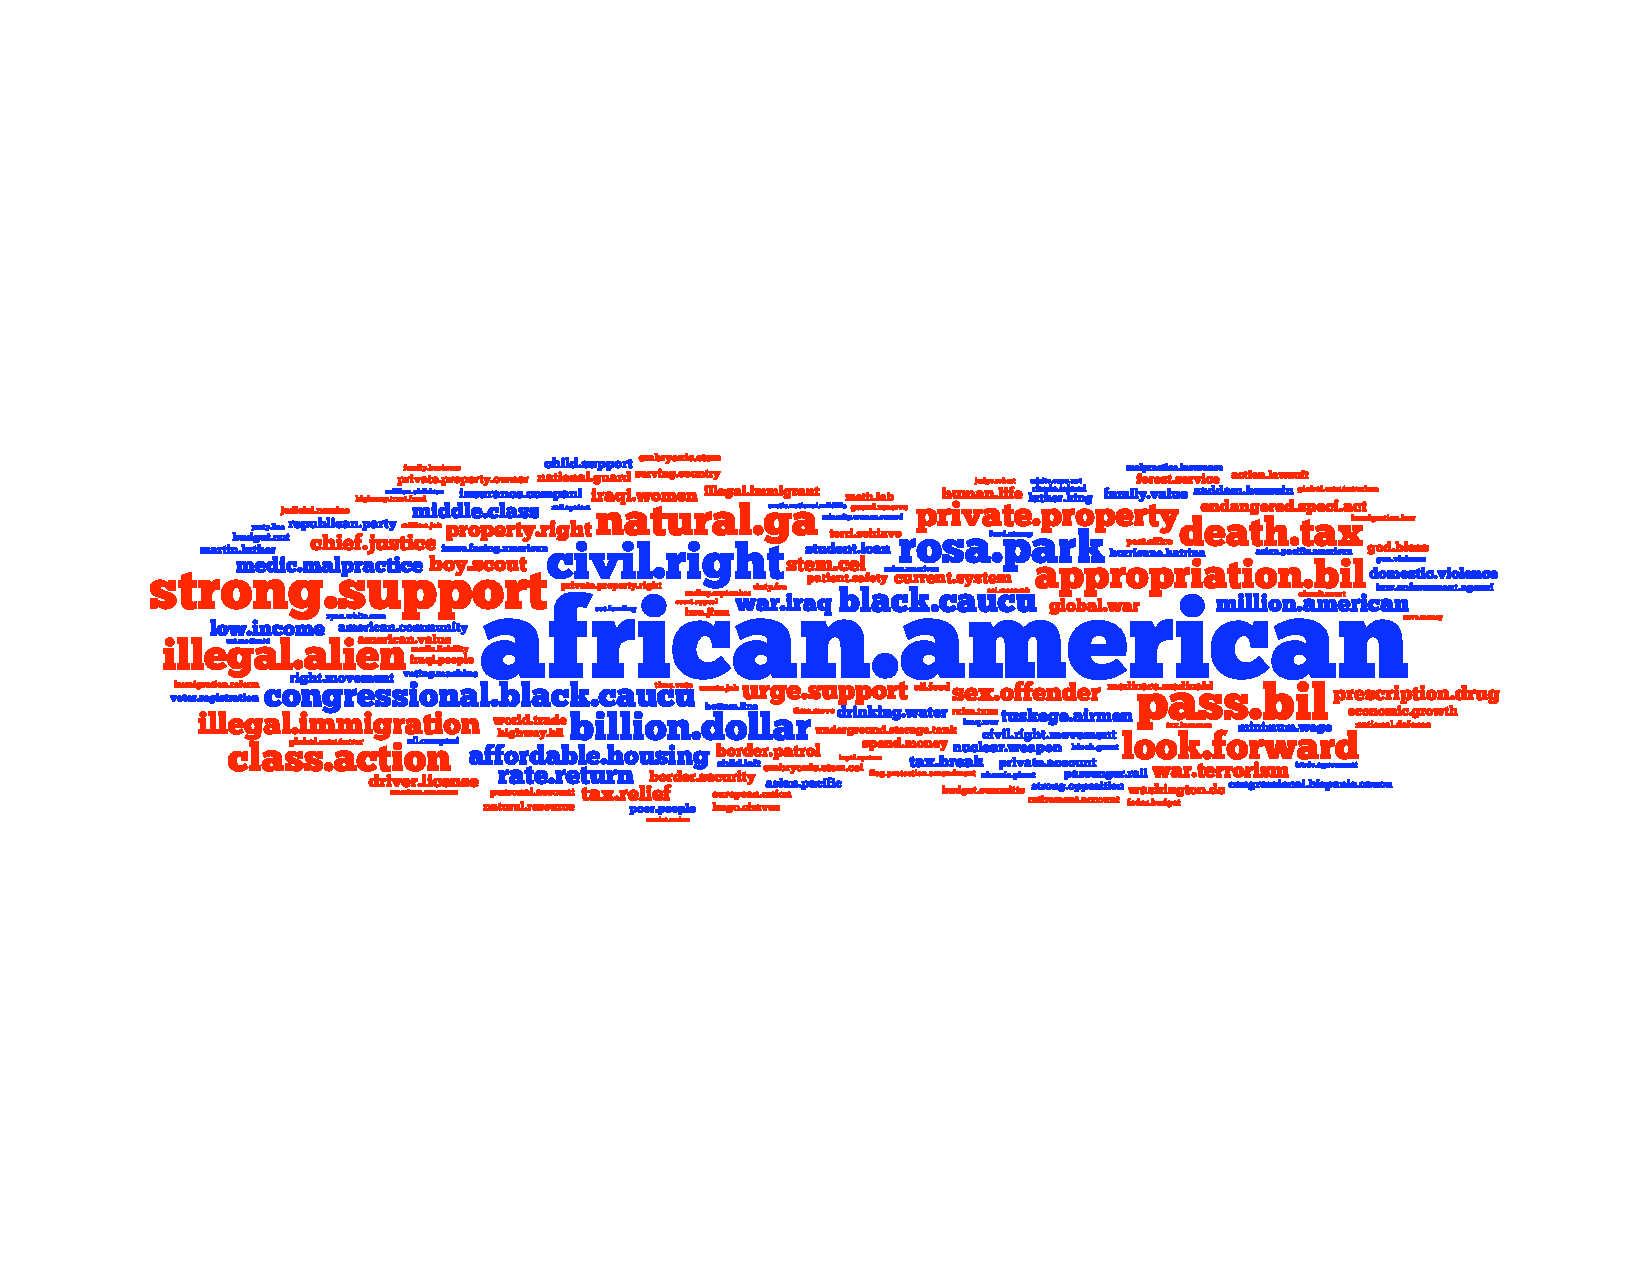
\includegraphics[width=4.5in]{figures/slantWrdl}
              
 \end{figure}

\begin{itemize}


\vskip .2cm
\item Colored by sign (\rd positive\bk, \bl negative\bk) \\ Size proportional to loading $\mr{cov}(f_j, y)$.\\

\vskip .2cm
\item Since $y$ is Republican vote-share, 
\begin{itemize}
\item Big positive is a right term and big
\item Negative is a left term.
\end{itemize}
\end{itemize}

\end{frame}
%----------------------------------------------------------------------%

\begin{frame}

\begin{center}
{\bf Slant measure for speakers in the 109th Congress}
\vskip -.5cm
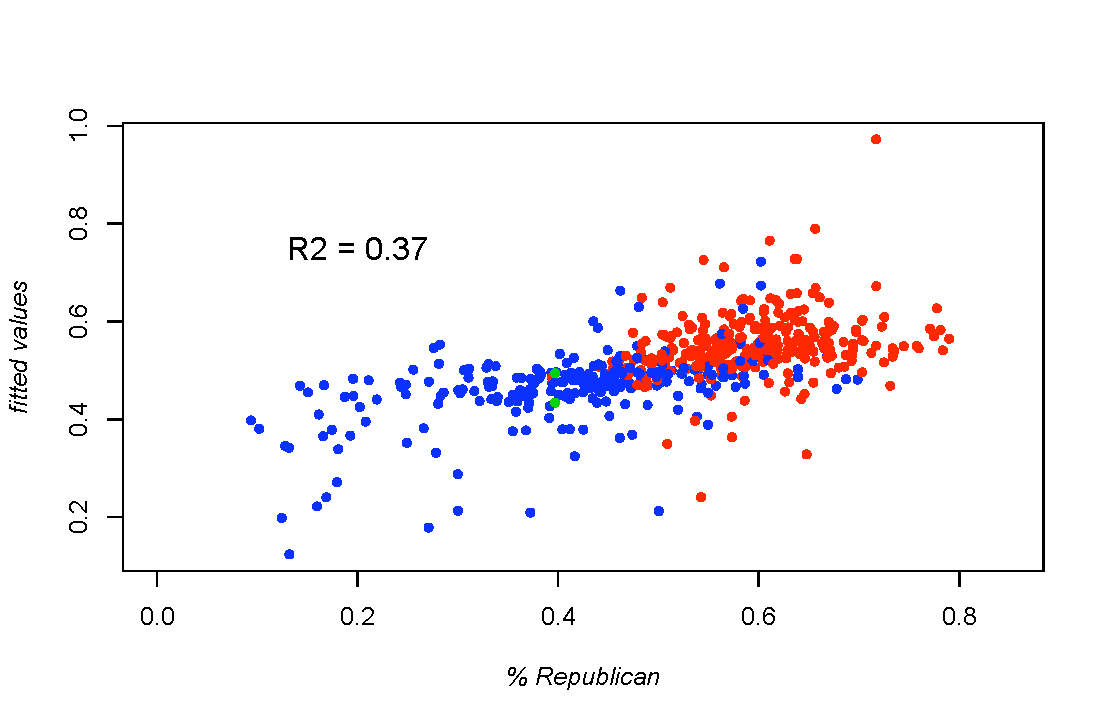
\includegraphics[width=4in]{figures/slant}\\
\end{center}

\vskip -.5cm
Democrats get low $z_\text{slant}$ and Republicans get high
$z_\text{slant}$.\\
\gr Do this for newspaper text and you'll get a similar picture

\end{frame}

%----------------------------------------------------------------------%
\begin{frame}[fragile]
\frametitle{Text as Data: The Big Picture}

\begin{itemize}


\item {\bf \theme Text is a vast source of data for business }
\medskip
\item It comes connected to interesting ``author'' variables 
\medskip
  \begin{itemize}
  \item What you buy, what you watch, your reviews
  \medskip
  \item Group membership, who you represent, who you email
  \medskip
  \item Market behavior, macro trends, the weather
  \end{itemize}

 
\item Opinion, subjectivity, etc.
\medskip
\item  Sentiment is {\it very} loosely defined:  Observables linked to the variables motivating language choice
\end{itemize}

\end{frame}

%----------------------------------------------------------------------%
\begin{frame}[fragile]
\frametitle{Text as Data: The Big Picture}

\begin{itemize}

\item {\bf \theme Text is also super high dimensional }

\medskip
\item And it gets higher dimensional as you observe more speech.


\medskip
\item Analysis of  phrase counts is the state of the art (hard to beat).


\item For example, occurrences by party for some partisan terms

\vskip .25cm
{\footnotesize
\begin{tabular}{|c|c|c|c|c|c|c}
Congress & State & Party & America & Death Tax & Estate Tax & $\cdots$
\\ \hline
\multirow{2}{*}{63} & \multirow{2}{*}{\sf NM} & {\sf dem}  & 108 &
  30 & 140 & \\ &
& {\sf gop}  & 100 &
  220 & 12  &
\end{tabular}}




\item Basic units of data

\begin{itemize}\bk
\item  doc-term count matrix $\bm{X}$ with rows $\bm{x}_i$.
\item  doc totals {\tt $\bm{m} = $ rowSums($\bm{X}$)} $=[m_1 \cdots m_n]$.
\item frequency matrix $\bm{F}=\bm{X}/\bm{m}$ with rows $\bm{f}_i$.
\end{itemize}

\end{itemize}

\end{frame}
%----------------------------------------------------------------------%
\section{Review
 \& Next Steps}
%----------------------------------------------------------------------%
\begin{frame}
\frametitle{Review \& Next Steps}
  
\begin{itemize} 
   \item XGBOOST
   \bigskip
   \item XGBOOST demo
   \bigskip
  \item Text as data
    \bigskip  
  \item  Next class:  More on text as data


\bigskip  
\item Questions? Questions about software? 

\end{itemize}
\end{frame}

%----------------------------------------------------------------------%
\section{Further Readings}
%----------------------------------------------------------------------%
\begin{frame}
\frametitle{Further Readings}

\begin{itemize}

  \item Chen, T., \& Guestrin, C. (2016, August). Xgboost: A scalable tree boosting system. In Proceedings of the 22nd acm sigkdd international conference on knowledge discovery and data mining (pp. 785-794).
  \medskip
  \item Chen, T., He, T., \& Benesty, M. (2018). XGBoost Documentation.
  \medskip
  \item Friedman, J., Hastie, T., \& Tibshirani, R. (2001). The elements of statistical learning (Vol. 1, No. 10). New York: Springer series in statistics.
  \medskip
  \item Taddy, M. (2019). Business data science: Combining machine learning and economics to optimize, automate, and accelerate business decisions. McGraw Hill Professional.

  
\end{itemize}

\end{frame}



%----------------------------------------------------------------------%
%----------------------------------------------------------------------%
\end{document}
%----------------------------------------------------------------------%
%----------------------------------------------------------------------%

